% !TeX root = RJwrapper.tex
\title{\pkg{DGLMExtPois}: Advances in Dealing with Over and Under-dispersion in a Double GLM Framework}
\author{by Antonio J. S\'{a}ez-Castillo, Antonio Conde-S\'{a}nchez and Francisco Mart\'{i}nez}

\maketitle

\abstract{
In recent years the use of regression models for under-dispersed count data, such as COM-Poisson or hyper-Poisson models, has increased. In this paper the \pkg{DGLMExtPois} package is presented. \pkg{DGLMExtPois} includes a new procedure to estimate the coefficients of a hyper-Poisson regression model within a GLM framework. The estimation process uses a gradient-based algorithm to solve a nonlinear constrained optimization problem. The package also provides an implementation of the COM-Poisson model, proposed by \citet{huang}, to make it easy to compare both models. The functionality of the package is illustrated by fitting a model to a real dataset. Furthermore, an experimental comparison is made with other related packages, although none of these packages allow you to fit a hyper-Poisson model.
}

%----------------------------------------------
% Section. Introduction
%----------------------------------------------

\section{Introduction}

The Poisson regression model is the most common framework for modeling count data, such as the number of accidents on a stretch of road, the number of visits to the doctor, the number of recreational or shopping trips, etc \citep{cameron_trivedi_2013,hilbe_2011,Winkelmann2008}. This model is constrained by its equi-dispersion assumption, that is, the mean is equal to the variance. However, this constraint is not usually met in real applications due to the existence of over-dispersion (the variance is greater than the mean) or under-dispersion (the variance is less than the mean). As over-dispersion is more common than under-dispersion, the former has received more attention from the research community.

Although the number of probabilistic models for count data affected by under-dispersion is not as high as that for over-dispersion, in recent years a significant effort has been made to provide suitable alternatives for applied researches to fit the data when the variance is below the mean. Generalized Poisson \citep{Consul92,Wang97, Famoye04, Zamani12, Grover15, sellers17}, Double Poisson \citep{Efron86, Zou13, sellers17}, Gamma count \citep{winkelmann95, Oh06, Lord10, daniels10, daniels11, Zeviani14, sellers17}, discrete Weibull \citep{McShane08, Ong15, klakattawi18, Yoo19} or Extended Poisson Process \citep{faddy11, smith16} are examples of models that may facilitate, in a regression context, a flexible dispersion structure wherein the Poisson assumption of equi-dispersion cannot be admitted because of the existence of factors that determine an excess or a shortfall of variability. In any case, Conway-Maxwell-Poisson, from now on CMP, is probably the most widely used model to fit data in the presence of under-dispersion. \citet{sellers10} presented a formulation of CMP in a regression context and demonstrated that the model could provide good fits to data not only affected by over-dispersion but also by under-dispersion, in the presence of covariates. The number of subsequent papers applying the model in different contexts is noteworthy \citep{sellers12, sellers17, CHATLA18, ABDELLA19}.

Nevertheless, the use of this CMP model has also been subject to criticism because of some limitations. First, there are some convergence problems in the calculation of the normalizing constant, the mean and the variance (since there are no closed expressions for them) \citep{francis12}. Second, and this is in our opinion its most important drawback, the original implementation of \citet{sellers10} and, therefore, all other applications based on it, consider a log-linear relationship between the covariates and the location parameter instead of the mean, so that the regression coefficients cannot be interpreted in terms of the effect size. In fact, some authors have considered a reparameterization looking for a central tendency parameter \citep{Guikema08, Lord10, francis12, Chanialidis2018}, although it is not really the mean.

Fortunately, \citet{huang} has recently implemented a new CMP parametrization where covariates are log-linearly related to the mean and the dispersion parameter, which has been continued in subsequent works \citep{huang19, ribeiro19, forthmann20}. The \pkg{mpcmp} package is based on the work of \citet{huang}. The hyper-Poisson regression model \citep{hp, lord, Saez-Castillo2017}, hereafter hP, provided an alternative that also presented both characteristics: on the one hand, covariates are introduced in the equation of the mean, commonly using a log-linear link, with regression coefficients measuring the effect size; on the other hand, the dispersion parameter may also be related to the covariates to facilitate a better fit of datasets which may be affected by over- or under-dispersion. Unfortunately, although the authors provided the necessary R code for a complete fit, the computational time needed to fit real data with medium or high sample size was so huge that its usefulness in real applications was very limited.

That is why our main aim in this paper is to improve the estimation procedure of the hP model. For this purpose, we have developed an R package, called \CRANpkg{DGLMExtPois}, in which the maximum likelihood optimization procedure has been accelerated. Of course, the package includes the  common methods and functions that allow for a complete analysis, including model diagnostics. The package also provides the \citet{huang} implementation of the CMP model that admits covariates in the dispersion parameter, mainly to facilitate comparisons between hP and CMP fits. In conclusion, what we want to demonstrate is the usefulness of CMP and hP models in a genuine GLM framework to test the significance and to assess the size effect of any explanatory variable on the mean value. At the same time, other explanatory variables may take part in the explanation of the dispersion structure, providing over- or under-dispersion depending on their different values.

%-------------------------------------------------------------------------
% Subsection. Comparison with other packages
%-------------------------------------------------------------------------
\subsection{Comparison with other packages}

There is currently no other package in R that estimates the hyper-Poisson model. There are two other packages that fit a COM-Poisson model: the \pkg{mpcmp} package that estimates the Huang's GLM implementation \citep{huang}, named $CMP_{\mu, \nu}$, and the \CRANpkg{COMPoissonReg} package that estimates the \citep{sellers10} model, denoted as $CMP_{\theta, \nu}$. The \pkg{DGLMExtPois} package also fits the $CMP_{\mu, \nu}$ model applying an optimization process similar to the one used in fitting $hP_{\mu, \gamma}$ models. The $CMP_{\mu, \nu}$ model was included in the \pkg{DGLMExtPois} package because, at the time the package was developed, no other package estimated this model with covariates in the dispersion parameter. However, recently the \pkg{mpcmp} package has included this feature. Table \ref{table:comparison} summarizes this comparison along with some additional features included in these packages for the analysis of the previously mentioned models.

\begin{table}[ht]
\centering
\begin{tabular}{llll}
\toprule
 & \pkg{DGLMExtPois} & \pkg{mpcmp} & \pkg{COMPoissonReg} \\ \midrule
$hP_{\mu, \gamma}$ model & Yes & No & No \\
$CMP_{\mu, \nu}$ model & Yes & Yes & No  \\
$CMP_{\theta, \nu}$ model & No & No & Yes  \\
Covariates in dispersion parameter & Yes & Yes & Yes \\
Zero inflated models & No & No & Yes \\
%Plots & Yes & Yes & No \\
\bottomrule
\end{tabular}
\caption{Feature comparison between packages \pkg{DGLMExtPois} (version 0.2.1), \pkg{mpcmp} (version 0.3.6) and \pkg{COMPoissonReg} (version 0.7.0).}
\label{table:comparison}
\end{table}

The remainder of this paper is structured as follows. First, we theoretically describe the $hP_{\mu, \gamma}$ model and the main estimation results for fitting data. Second, we do the same for the $CMP_{\theta, \nu}$ and  $CMP_{\mu, \nu}$ models. After that, we describe the \pkg{DGLMExtPois} package, illustrating the fit of a real dataset. Next, we include a comparison of fits of $hP_{\mu, \gamma}$, $CMP_{\theta, \nu}$ and $CMP_{\mu, \nu}$ models with different well-known datasets. Finally, we carry out a simulation to assess the performance of the estimates and standard errors of the $hP_{\mu, \gamma}$ model and discuss the optimization process.

%----------------------------------------------
% Section. The hP model
%----------------------------------------------
\section{The $hP_{\mu, \gamma}$ model}

Let us consider $Y$ as count variable of a hyper-Poisson distribution, whose probability mass function is \citep{hp}
\begin{equation}
    P\left[Y = y \right] = \frac{1}{_{1}F_{1}\left(1, \gamma; \lambda \right)} \frac{\lambda^{y}} {\left(\gamma \right)_{y}}, \qquad \lambda, \gamma > 0, \label{hp}
\end{equation}
where
\[
_{1}F_{1}\left(1, \gamma; \lambda \right) = \sum_{y = 0}^{\infty} \frac{\lambda^{y}}{\left(\gamma\right)_{y}},
\]
and $(\gamma)_y = \Gamma(\gamma + y) / \Gamma(\gamma)$. The parameter $ \gamma $ is known as the dispersion parameter because for $ \gamma > 1 $ the distribution is over-dispersed and for $ \gamma < 1 $ it is under-dispersed (for $ \gamma = 1 $ we have the Poisson distribution).

Let $\left(X_1, \dots, X_{q_1} \right) \in \mathbb{R}^{q_1}$ and $\left(Z_1, \dots, Z_{q_2} \right) \in \mathbb{R}^{q_2}$ be two sets of explanatory variables or covariates. These two sets can be disjoint or overlapping (they can even be equal). In an $hP_{\mu, \gamma}$ GLM model, $Y$ follows a hyper-Poisson distribution whose mean, $\mu$, and dispersion parameter, $\gamma$, are functions of the covariates. In our case, log-linear relations are always considered, so $\log \mu = \mathbf{X} \boldsymbol{\beta}$ and $\log \gamma = \mathbf{Z} \boldsymbol{\delta}$, such that $ {\bf X} = \left(1, X_1, \dots, X_{q_1} \right) $ and $ {\bf Z} = \left(1, Z_1, \dots, Z_{q_2} \right) $ the design matrices, and $\boldsymbol{\beta}' = \left(\beta_0, \beta_1, \dots, \beta_{q_1} \right)$ and $\boldsymbol{\delta}' = \left(\delta_0, \delta_1, \dots, \delta_{q_2} \right)$ the regression coefficients. Moreover, the parameter $ \lambda $ is the solution of
\begin{equation}
\mu = \exp (\mathbf{X} \boldsymbol{\beta}) = \sum_{y = 0}^{\infty} y \times P[Y = y] \label{eq:link}.
\end{equation}
\citet{hp} include a study of the relationship between $\lambda(\mu, \gamma)$, which can be interpreted as a location parameter, and the mean, $\mu$, for a wide range of $\gamma$ values.

The hP distribution belongs to the exponential family only for a given $\gamma$ value. This justifies that the $hP_{\mu, \gamma}$ model can be considered as a member of the GLM family. Moreover, since the model also allows you to introduce covariates in the dispersion parameter, we refer to it as \dfn{double GLM}, although we highlight that the hP distribution does not properly belong to the exponential family for unknown $\gamma$.

The previous definition of the $hP_{\mu, \gamma}$ model \citep{hp} was based on an alternative equation, different from (\ref{eq:link}). Concretely, the authors proposed a closed equation that involves the mean, the variance and the normalizing constant. The substitution of the previous equation by equation (\ref{eq:link}) and the change of the optimization algorithm have been the key points in the great reduction of the computational time needed to fit real data provided by the \pkg{DGLMExtPois} package.

To this end, we consider maximum likelihood for the estimation of the regression coefficients. Letting $(Y_i, X_{1i}, \dots, X_{q_1i}, Z_{1i}, \dots, Z_{q_2i}) $, $ i = 1, ... , n$, be a random sample, the log-likelihood is given by
\begin{equation}\label{logverhp}
% \begin{split}
    l_{hP}\left(\beta, \delta\right) = \sum_{i = 1}^n \left\{ Y_i  \log\left(\lambda\left(\mu_i, \gamma_i\right)\right) - \log\left(\Gamma\left(\gamma_i + Y_i\right)\right) + \log\left(\Gamma\left(\gamma_i\right)\right) - \log(_{1}F_{1} \left(1, \gamma_i; \lambda\left(\mu_i, \gamma_i\right) \right)) \right\}
% \end{split}
\end{equation}
where
\[
\log \mu_i = \mathbf{x}_i' \boldsymbol{\beta}
\]
and
\[
\log \gamma_i = \mathbf{z}_i' \boldsymbol{\delta},
\]

being $ \mathbf{x}_i' $ and $ \mathbf{z}_i' $ the $i$th row of the design matrices and each $\lambda_i=\lambda\left(\mu_i, \gamma_i\right)$ is a solution of (\ref{eq:link}) for a given $\mu_i$ and $\gamma_i$. This converts the maximum likelihood procedure into a nonlinear constrained optimization problem where the objective function is $(n + q_1 + q_2 + 2)$-dimensional, depending on $n$ nuisance $\lambda_i$ parameters, $q_1 + 1$ regression coefficients for the mean, $\boldsymbol{\beta}$, and $q_2 + 1$ regression coefficients for the dispersion parameter, $\boldsymbol{\delta}$, and it is constrained by $n$ non-linear equations from (\ref{eq:link}). We have implemented it using a sequential quadratic programming (SQP) gradient-based algorithm \citep{kraft1994algorithm}; concretely, the NLOPT\_LD\_SLSQP algorithm included in the \CRANpkg{nloptr} package \citep{nloptr}.

In the implementation, it was necessary to compute the gradient of the objective function and the gradient of restriction \eqref{eq:link}, in which the reparameterization of $ \lambda' = \log \lambda $ has been considered to ensure the positivity of $ \lambda $. These expressions have been included in the appendix.

Moreover, the following results are verified:
\begin{res}\label{res_beta}
For a sample $ Y_1, \dots, Y_n $ from a hyper-Poisson the score function with respect to $ \boldsymbol{\beta} $ is
\begin{equation}\label{scorebeta}
    S_{\boldsymbol{\beta}} = \frac{\partial l_{hP}}{\partial \boldsymbol{\beta}} = \sum_{i=1}^n \frac{Y_i - \mu_i}{V\left(\mu_i,\gamma_i\right)} \mu_i \mathbf{x}_i'
\end{equation}
where $ V\left(\mu_i,\gamma_i\right) $ is the variance of an $hP$ with a probability mass function given by \eqref{hp}, which depends on $\mu_i$ and $\gamma_i$. This way, the MLE of $\boldsymbol{\beta}$ can be characterized as the solution to the usual GLM score equations.
\end{res}

\begin{res}\label{res_delta}
For a sample of size  $ n $ from a hyper-Poisson it is verified that
\begin{equation}\label{scoredelta}
    S_{\boldsymbol{\delta}}= \frac{\partial l_{hP}}{\partial\boldsymbol{\delta}} = \sum_{i=1}^n \left\{\left(Y_i - \mu_i\right)\frac{Cov \left[Y_i \psi\left(\gamma_i+ Y_i\right) \right]}{V\left(\mu_i,\gamma_i\right)} - \psi\left(\gamma_i+Y_i\right) + E \left[ \psi\left(\gamma_i+Y_i\right) \right]  \right\} \gamma_i \mathbf{z}_i'
\end{equation}
where $\psi()$ is the digamma function.
\end{res}

The proof is included in the appendix. We have obtained estimates of the standard errors of the maximum likelihood estimators of $\boldsymbol{\beta}$ and $\boldsymbol{\delta}$ based on Cramer-Rao bound, which requires a closed expression of the Fisher information matrix. %If we denote
%\[
%S_{\beta} = \frac{d}{d\beta} P[Y = y \mid _{X = x, Z = z}]
%\]
%and
%\[
%S_{\delta} = \frac{d}{d\delta} P[Y = y \mid _{X = x, Z = z}],
%\]
%then the Fisher information matrix in the sample may be approximated by
\begin{res}\label{inf_mat}
The Fisher information matrix in the sample can be approximated by
\begin{align*}
    I_n\left(\hat{\beta},\widehat{\boldsymbol{\delta}}\right) = \left(
    \begin{array}{c|c}
    \displaystyle{\sum_{i=1}^n} E\left[S_{\widehat{\boldsymbol{\beta}}}S_{\widehat{\boldsymbol{\beta}}}'\right] & 0 \\
    \hline
    0 & \displaystyle{\sum_{i=1}^n} E\left[S_{\widehat{\boldsymbol{\delta}}}S_{\widehat{\boldsymbol{\delta}}}'\right]
\end{array}
    \right)
\end{align*}
where
\[
\sum_{i=1}^n E\left[S_{\boldsymbol{\beta}}S_{\boldsymbol{\beta}}'\right] = \sum_{i=1}^n \frac{\mu_i^2}{V\left(\mu_i,\gamma_i\right)} \mathbf{x}_i \mathbf{x}_i'
\]

\[
\sum_{i=1}^n E\left[S_{\boldsymbol{\delta}}S_{\boldsymbol{\delta}}'\right] = \sum_{i=1}^n \left[ Var\left(\psi\left(\gamma_i + Y_i\right)\right) - \frac{Cov\left(Y_i, \psi\left(\gamma_i + Y_i\right)\right)}{V\left(\mu_i,\gamma_i\right)} \right] \gamma_i^2 \mathbf{z}_i \mathbf{z}_i'.
\]
are evaluated in the maximum likelihood estimates, $\widehat{\boldsymbol{\beta}}$ and $\widehat{\boldsymbol{\delta}}$. The proof is included in the appendix.
\end{res}

Standard error estimates would appear in the diagonal of the inverse of $I_n\left(\widehat{\boldsymbol{\beta}},\widehat{\boldsymbol{\delta}}\right)$. We have not experienced any difficulties in this computation, nor in the inversion of $\sum_{i=1}^n E\left[S_{\beta}S_{\beta}'\right]$. In contrast, $\sum_{i=1}^n E\left[S_{\boldsymbol{\delta}}S_{\boldsymbol{\delta}}'\right]$ is sometimes nearly singular, so the standard errors of $\widehat{\boldsymbol{\delta}}$ are not always estimated and, sometimes, are quite large. That is the reason why we recommend assessing the significance of covariates included in $\mathbf{Z}$ using the likelihood ratio test (LRT) instead of the Wald test, since it requires a convenient estimation of $\widehat{\boldsymbol{\delta}}$ standard errors.

%-------------------------------------------------------------------------
% Section. The CMP models
%-------------------------------------------------------------------------
\section{The $CMP_{\theta, \nu}$ and $CMP_{\mu, \nu}$ models}

The probabilities of the CMP distribution are given by
\begin{equation}
    P\left[Y = y \right] = \frac{1}{Z\left(\theta, \nu \right)} \frac{\theta^{y}} {\left(y!\right)^{\nu}}, \qquad \theta, \nu > 0, \label{cmp}
\end{equation}
with
\[
Z\left(\theta, \nu\right) = \sum_{y = 0}^{\infty} \frac{\theta^{y}}{\left(y!\right)^{\nu}}.
\]
Here, $\nu < 1$ corresponds to over-dispersion and $\nu > 1$ to under-dispersion. The distribution belongs to the bi-parametric exponential family \citep{huang}. In this distribution, $\theta$ is a location parameter with a similar role to $\lambda$ for the hP distribution. It is worth emphasizing that $\theta$ is \textit{not} a mean, see for example \citet{francis12} for the exact relationship between $ \theta $ and $ \mu $. 

%If $Y$ is again the response count variable and $\left(X_1, \dots, X_{q_1} \right) \in \mathbb{R}^{q_1}$ and $\left(Z_1, \dots, Z_{q_2} \right) \in \mathbb{R}^{q_2}$ are two sets of explanatory variables, we denote as $CMP_{\theta, \nu}$ the model wherein
If $Y$ is again the response count variable and $ \mathbf{X} $ and $ \mathbf{Z} $ are defined as above, then we denote as $CMP_{\theta, \nu}$ the model wherein
\[
\log \theta =  \mathbf{X} \boldsymbol{\beta}
\]
and
\[
\log \nu = \mathbf{Z} \boldsymbol{\delta}.
\]
This is the model with constant $\nu$ defined by \citet{sellers10}, later extended to consider covariates in the $\nu$ equation \citep{sellers12, CHATLA18}. In contrast, the model defined by \citet{huang} is given as

\[
\log \mu =  \mathbf{X} \boldsymbol{\beta}
\]
and

\[
\log \nu = \mathbf{Z} \boldsymbol{\delta},
\]
where additionally equation \eqref{eq:link} must be verified for each observation, and the probabilities in \eqref{cmp}. We denote this model as $CMP_{\mu, \nu}$.

Estimation and inference for the $CMP_{\theta, \nu}$ is described, for example, in \citet{sellers10}. The \pkg{COMPoissonReg} package \citep{COMPoissonReg} provides adequate methods and functions to estimate such a model. \citet{huang} also provides theoretical results describing the procedure to obtain estimates of $\boldsymbol{\beta}$ and $\boldsymbol{\delta}$ using maximum-likelihood and related inference results for $CMP_{\mu, \nu}$, which are included in the \pkg{mpcmp} package.

%-------------------------------------------------------------------------
% Section. The DGLMExtPois package
%-------------------------------------------------------------------------
\section{The \pkg{DGLMExtPois} package}

At present, packages such as \pkg{COMPoissonReg} provide what a practitioner commonly requires to fit real data. Our main criticism, as we have mentioned in the introduction section, is that $\boldsymbol{\beta}$ regression coefficients cannot be interpreted in terms of the effect size. In this sense, \pkg{mpcmp} is, in our opinion, a better proposal for practitioners looking for a clearer interpretation of the $\boldsymbol{\beta}$ regression coefficients in relation to the effect of each explanatory variable on the mean of the response variable.

In this context, what  the \pkg{DGLMExtPois} package provides is, first, a much faster implementation of the $hP_{\mu, \gamma}$ model than the previous existing R code and, second, our own implementation of $CMP_{\mu, \nu}$ to facilitate the comparison of the models.

\pkg{DGLMExtPois} has been created by trying to reproduce the syntax of GLM fits. Thus, functions \code{glm.hP} and \code{glm.CMP} provide the corresponding fits for $hP_{\mu, \gamma}$ and $CMP_{\mu, \nu}$, respectively. There are also \code{print} and \code{summary} methods to visualize the fitted models and \code{AIC}, \code{confint}, \code{predict}, \code{residuals} and \code{plot} methods to evaluate the goodness of fit, obtain confidence intervals of $\boldsymbol{\beta}$ regression coefficients, predictions, residuals and some associated plots, such as QQ-plots and simulated envelopes. The package additionally incorporates \code{expected}, a function which calculates the marginal probabilities of the $Y$ variable, and \code{lrtest} to get the likelihood ratio test in nested models. Other functions are provided, for example, to work with  probabilities of CMP and hP distributions. A brief description of the main functions in the package is given in Table \ref{tab_functions}.
\begin{table}[]
    \centering
    \begin{tabular}{ll}
    \toprule
     Function & Description \\ \midrule
     \code{glm.hP} & Fits an $hP_{\mu, \gamma}$ model \\
     \code{glm.CMP} & Fits an $CMP_{\mu, \nu}$ model \\
     \code{lrtest} & Likelihood ratio chi-squared test \\
     \code{residuals} & Extracts model residuals (Pearson, response and quantile) and produces \\
     & a simulated envelope \\
     \code{fitted} & Fitted values of the model \\
     \code{plot} & Plot of residuals against fitted values and a Normal Q-Q plot \\
     \code{predict} & Predictions \\
     \code{confint} & Confidence intervals for $\boldsymbol{\beta}$ regression coefficients \\
     \code{dhP} & Probability mass function for an $hP$ distribution \\
     \code{phP} & Distribution function for an $hP$ distribution \\
     \code{rhP} & Random generation for an $hP$ distribution\\
     \code{hP\_expected} & Expected frequencies for $hP_{\mu, \gamma}$ model \\
     \code{CMP\_expected} & Expected frequencies for $CMP_{\mu, \nu}$ model \\
    \bottomrule
    \end{tabular}
    \caption{Main functions in the \pkg{DGLMExtPois} package.}
    \label{tab_functions}
\end{table}

\subsection{Installation}

As usual, you can install the \pkg{DGLMExtPois} package from CRAN with the code:

\begin{example}
install.packages("DGLMExtPois")
\end{example}

You may encounter problems on Windows operating systems if you are not logged in with administrator rights due to the strong dependency on the \pkg{nloptr} package.

%-------------------------------------------------------------------------
% Section. Numerical examples
%-------------------------------------------------------------------------
\section{Numerical examples}

In this section the main methods and functions in the package are illustrated by fitting a real dataset. Also, several well-known datasets in regression on count variables have been used to compare \pkg{COMPoissonReg} and \pkg{DGLMExtPois} in terms of goodness of fit, computational times and reliability. Finally, some guidelines are given on the optimization process for estimating the models.

\subsection{Example of application}

The dataset originates from research on customer profiles for a household supplies company. An observation corresponds to census tracts within 10-mile radius around a certain store. The response variable is the number of customers of each census tract who visit the store and the explanatory variables are related to relevant demographic information for each tract. The dataset was analyzed in \citet{Neter1996} as an example of a Poisson regression model, since it is a classic instance of equidispersed count data. They consider the number of housing units (\code{nhu}), the average income in dollars (\code{aid}), the average housing unit age in years (\code{aha}), the distance to the nearest competitor in miles (\code{dnc}) and the distance to store in miles (\code{ds}) as covariates. Here, we consider this dataset to illustrate the performance of \pkg{DGLMExtPois} fitting models with all the explanatory variables in the mean equation and one of them, \code{dnc}, in the dispersion parameter equation. The dataset is also analyzed in \citep{Bonat} considering the Extended Poisson-Tweedie distribution, but they also obtain an equidispersed distribution.

First, we fit a Poisson regression model, an $hP_{\mu, \gamma}$ model and a $CMP_{\mu, \nu}$ model without explanatory variables in the dispersion parameter:

\begin{example}
library(DGLMExtPois)
formula.loc   <- ncust ~ nhu + aid + aha + dnc + ds # Mean formula
formula.disp0 <- ncust ~ 1                          # Dispersion parameter formula

pois <- glm(formula.loc, data = CustomerProfile, family = 'poisson')

hp0  <- glm.hP(formula.loc, formula.disp0, data = CustomerProfile)
cmp0 <- glm.CMP(formula.loc, formula.disp0, data = CustomerProfile)
c(AIC(pois), AIC(hp0), AIC(cmp0))
[1] 571.0243 571.7983 573.0006
\end{example}

The functions \code{glm.hP} and \code{glm.CMP} return S3 objects of classes \code{"glm\_hP"} and \code{"glm\_CMP"}, respectively, with information on the fitted models. The most suitable model according to AIC is Poisson. The fits for these models, shown in Table \ref{tab_constant_dispersion}, indicate that there is equidispersion. In fact, if the LRT is carried out to determine whether the dispersion parameter is equal to 1 (Poisson model), the hypothesis is not rejected:

\begin{table}
    \centering
%    \small
    \begin{tabular}{@{}ccccccc@{}}
    \toprule
    & \multicolumn{2}{c}{Poisson} & \multicolumn{2}{c}{$hP_{\mu, \gamma}$} & \multicolumn{2}{c}{$CMP_{\mu, \nu}$} \\     \cmidrule{2-7}
    &            Estimate & Std. Error  &  Estimate & Std. Error & Estimate & Std. Error \\ \midrule
(Intercept) & 2.9424 & 0.2072 & 2.9465 & 0.2155 & 2.9426 & 0.2051 \\
nhu         & 0.0606 & 0.0142 & 0.0600 & 0.0147 & 0.0606 & 0.0141 \\
aid         &-0.0117 & 0.0021 &-0.0115 & 0.0022 &-0.0117 & 0.0021 \\
aha         &-0.0037 & 0.0018 &-0.0038 & 0.0018 &-0.0037 & 0.0018 \\
dnc         & 0.1684 & 0.0258 & 0.1662 & 0.0269 & 0.1683 & 0.0255 \\
ds          &-0.1288 & 0.0162 &-0.1285 & 0.0168 &-0.1288 & 0.0160 \\ \midrule
(Intercept) &        &        & 0.6229 & 0.6574 & 0.0219 & 0.1407 \\ \bottomrule
    \end{tabular}
    \caption{Estimation of coefficients and standard errors for fitted models with a constant dispersion parameter. The last row is the estimation of $\delta_0$ and its standard error.}
    \label{tab_constant_dispersion}
\end{table}

\begin{example}
lrt_hp <- -2 * (hp0$logver + logLik(pois)[1])
pchisq(lrt_hp,1, lower.tail = FALSE)
[1] 0.2681826
lrt_cmp <- -2 * (cmp0$logver + logLik(pois)[1])
pchisq(lrt_cmp,1, lower.tail = FALSE)
[1] 0.8777006
\end{example}

However, if we introduce covariates in the dispersion parameter we find that the equidispersion hypothesis is rejected, hence the importance of being able to include variables that determine a different variability in the model. We have checked that none of the explanatory variables lead to a statistically significant improvement in the likelihood of the $CMP_{\mu, \nu}$ model when they are introduced as covariates for the dispersion parameter. That is why, from now on, we concentrate on how to use the package with the $hP_{\mu, \gamma}$ model.

Let us now consider a new $hP_{\mu, \gamma}$ model with \code{dnc} in the dispersion parameter equation:

\begin{example}
formula.disp1 <- ncust ~ dnc        # New dispersion parameter formula
hp1           <- glm.hP(formula.loc, formula.disp1, data = CustomerProfile)
\end{example}

The \code{summary} method provides, as usual, the regression coefficient estimates, their standard errors, the corresponding t-statistics and p-values and other details about the model:

\begin{example}
summary(hp1)

Call:
glm.hP(formula.mu = formula.loc, formula.gamma = formula.disp1,
    data = CustomerProfile)

Mean model coefficients (with log link):
             Estimate Std. Error z value Pr(>|z|)
(Intercept)  2.996083   0.204212  14.671  < 2e-16 ***
nhu          0.054473   0.013960   3.902 9.54e-05 ***
aid         -0.010930   0.002068  -5.285 1.26e-07 ***
aha         -0.003631   0.001751  -2.074   0.0381 *
dnc          0.156249   0.026233   5.956 2.58e-09 ***
ds          -0.128101   0.015636  -8.193 2.55e-16 ***
---
Signif. codes:  0 ‘***’ 0.001 ‘**’ 0.01 ‘*’ 0.05 ‘.’ 0.1 ‘ ’ 1

Dispersion model coefficients (with logit link):
            Estimate Std. Error z value Pr(>|z|)
(Intercept)    4.749      2.416   1.965   0.0494 *
dnc           -2.782      2.272  -1.224   0.2208
---
Signif. codes:  0 ‘***’ 0.001 ‘**’ 0.01 ‘*’ 0.05 ‘.’ 0.1 ‘ ’ 1

AIC: 568.1
\end{example}

The Wald test assesses whether the \code{dnc} variable is significant or not for the dispersion parameter. In any case, as previously mentioned, we also used the LRT to confirm the adequacy of \code{hp1} versus the \code{hp0} model, with a significance level of 0.05, resulting in the rejection of the constant dispersion hypothesis:

\begin{example}
lrtest(hp0, hp1)
Statistics: 5.668851
Degrees of freedom: 1
p-value: 0.01726877
\end{example}

Since the dispersion parameter in the \code{hp1} model depends on \code{dnc}, its values may determine over- or under-dispersion. It is interesting to note that low values of the \code{dnc} variable show over-dispersion while  high values show under-dispersion. Specifically, the point at which the change occurs is 1.7069. There are  24 out of the 110 cases with $\gamma_i > 1$, and thus over-dispersed, underlying $hP(\mu_i, \gamma_i)$ distributions, see  Figure \ref{fig:dispersion}. The plot suggests a certain correlation between under-dispersion and high response variable values.

\begin{figure}[h]
	\centering
	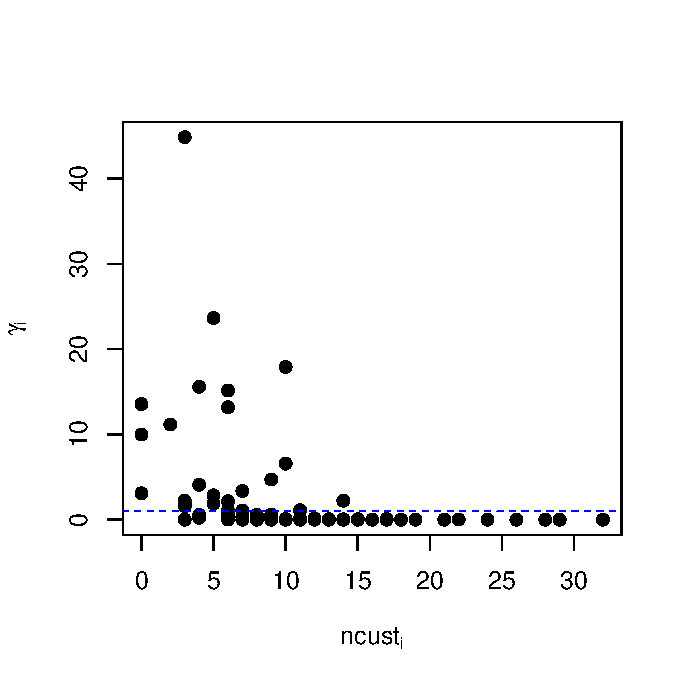
\includegraphics[scale=0.6]{dispersion.pdf}
	\caption{Value of the dispersion parameter according to the response variable. The points above the dashed line are greater than 1, so the distribution is over-dispersed. These points occur for low values of the response variable.}
	\label{fig:dispersion}
\end{figure}

\begin{example}
plot(CustomerProfile$ncust, hp1$gamma,
     xlab = expression(ncust[i]),
     ylab = expression(gamma[i]),
     pch = 19
)
abline(h = 1, lty = "dashed", col = "blue")
\end{example}

The \code{plot} method provides two classical plots for the model diagnostics: residuals against fitted values and a normal QQ-Plot. In relation to the residuals, Pearson, deviance and response residuals are offered, although here we only calculate the Pearson type (top row of Figure \ref{fig:diagnostics}). The package also provides the possibility to compare in a barplot the observed and expected marginal frequencies of the response variable with the \code{hP\_expected} and the \code{CMP\_expected} functions (Figure \ref{fig:diagnostics:c}). Finally, the diagnostic can be completed by a simulated envelope for the residuals to assess the accuracy of the model on the entire dataset \citep{atkinson,GARAY}. The \code{residuals} method provides this diagnostic tool, and in Figure \ref{fig:diagnostics:d} the cases for which the model assumptions are rejected are highlighted in red. In this case there are 5 observations that fall outside the envelope, therefore there is no evidence against the adequacy of the model.

\begin{figure}
	\centering
	\begin{subfigure}{0.475\textwidth}
		\centering
		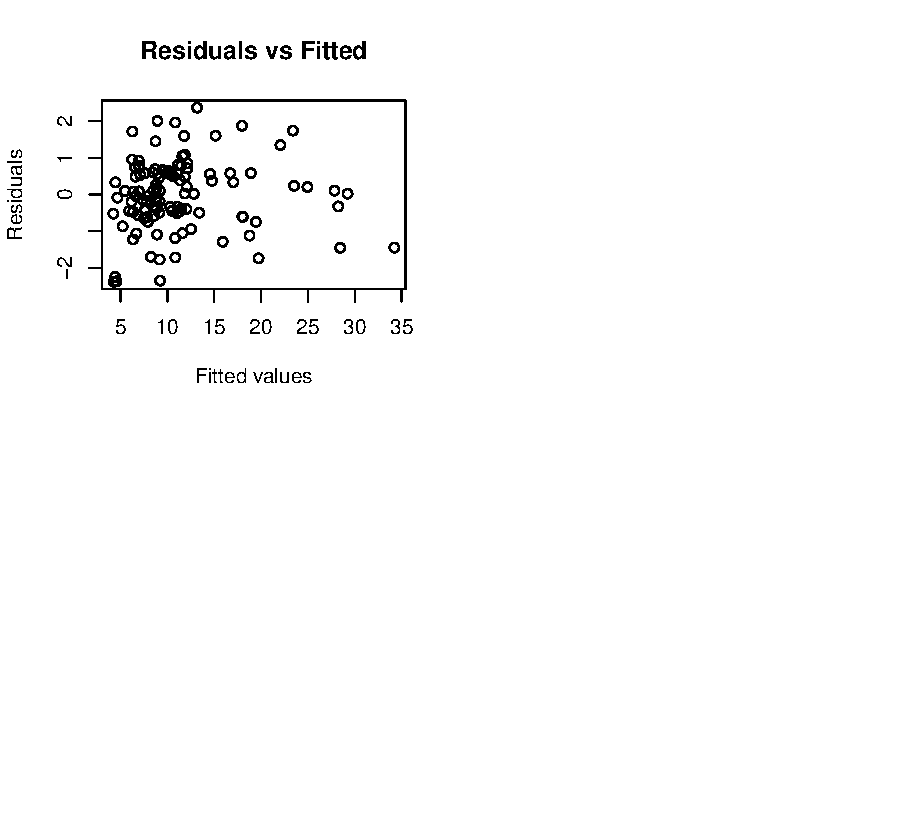
\includegraphics[width=\textwidth]{diagnostics_a.pdf}
		\caption{Residuals versus fitted values.}
		\label{fig:diagnostics:a}
	\end{subfigure}
	\hfill
	\begin{subfigure}{0.5\textwidth}
		\centering
		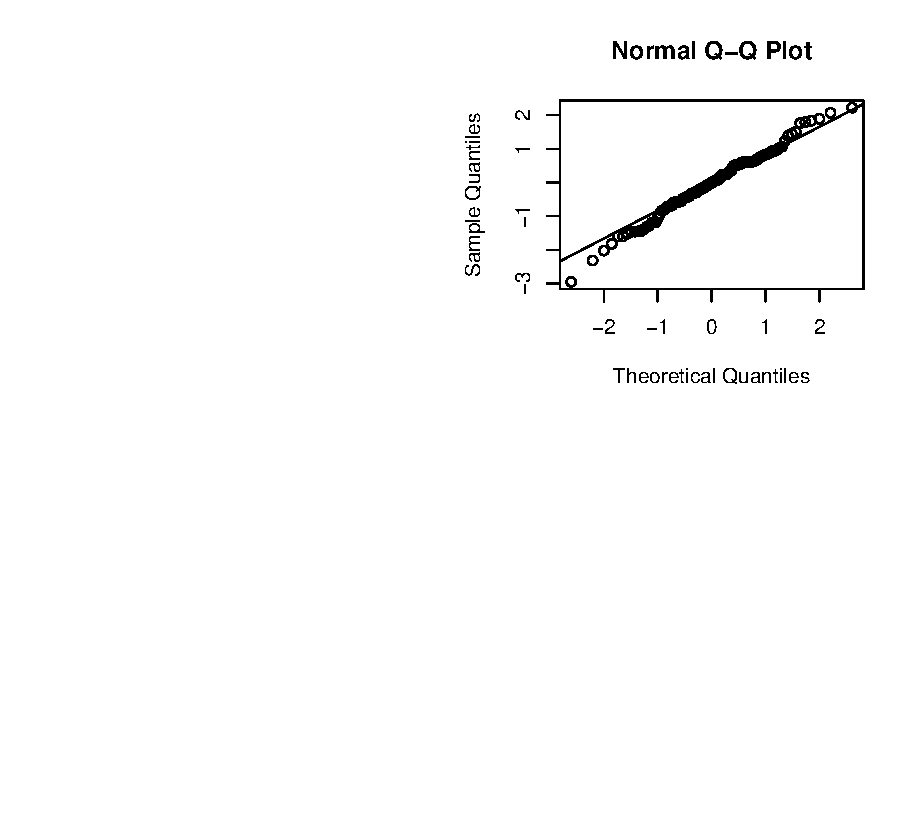
\includegraphics[width=\textwidth]{diagnostics_b.pdf}
		\caption{Normal QQ plot.}
		\label{fig:diagnostics:b}
	\end{subfigure}
	
	\begin{subfigure}{0.5\textwidth}
		\centering
		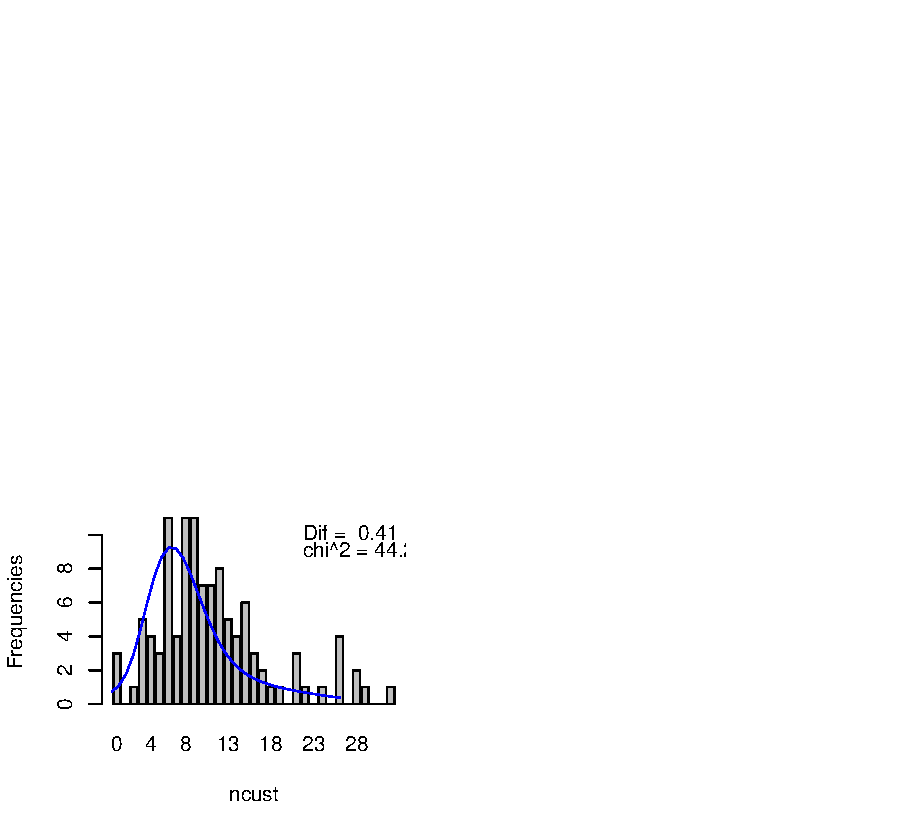
\includegraphics[width=\textwidth]{diagnostics_c.pdf}
		\caption{Bar\_plot for the observed marginal frequencies. The blue line represents the expected marginal frequencies for the response variable.}
		\label{fig:diagnostics:c}
	\end{subfigure}
	\hfill
	\begin{subfigure}{0.475\textwidth}
		\centering
		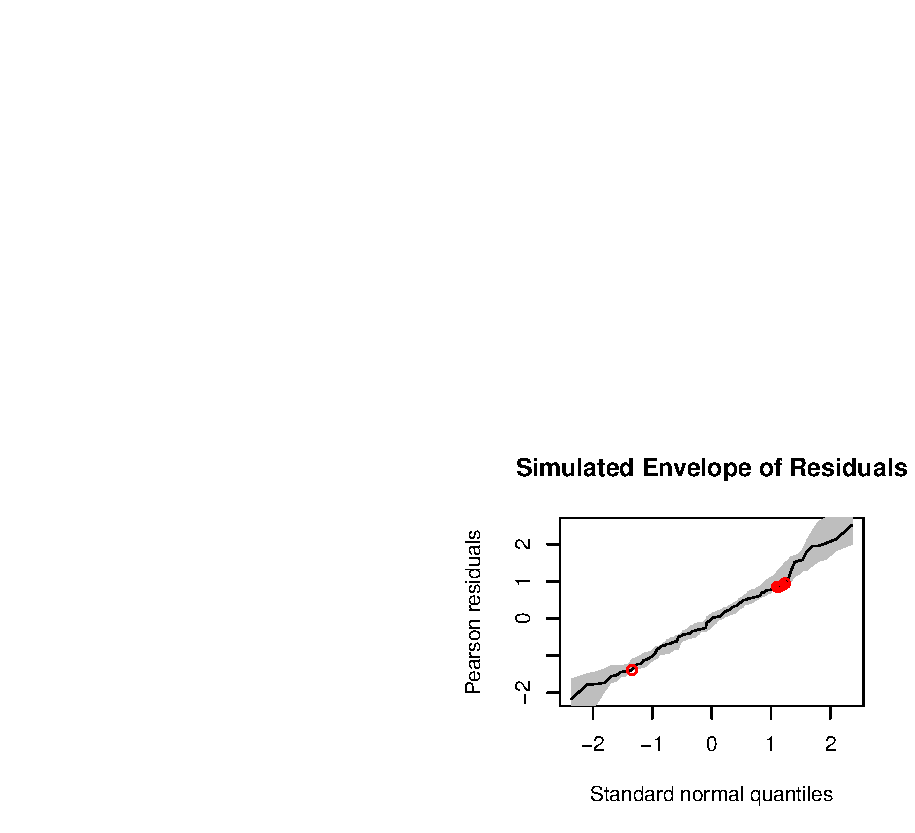
\includegraphics[width=\textwidth]{diagnostics_d.pdf}
		\caption{Normal QQ plot with simulated envelopes of residuals. The shaded gray region contains 95\% of the simulated points for each observation.}
		\label{fig:diagnostics:d}
	\end{subfigure}
	\caption{Regression diagnostics. The plots do not show evidence against the adequacy of the model.}
	\label{fig:diagnostics}
\end{figure}


\begin{example}
par(mfrow = c(2, 2))
set.seed(21)
plot(hp1) # Residuals against fitted values and normal QQ plot

# Observed and expected marginal frequencies
expec_hp <- hP_expected(hp1)
barplot(expec_hp$observed_freq[0:33], xlab = "ncust", ylab = "Frequencies")
lines(expec_hp$frequencies[1:33], x = c(0:32), col = "blue")
text(x = c(25, 25), y = c(10, 9), c(paste("Dif = ", round(expec_hp$dif, 2)),
     paste(expression(chi ^ 2), "=", round(expec_hp$chi2, 2))), pos = 4)

# Envelope
r1 <- residuals(hp1, envelope = TRUE)
envelope_down <- apply(r1$sim_residuals, 1, min)
envelope_up <- apply(r1$sim_residuals, 1, max)
weirds <- which(r1$residuals < envelope_down | r1$residuals > envelope_up)
score_weirds <- qnorm(weirds / 111)
points(score_weirds, r1$residuals[weirds], col = "red")
\end{example}

\subsection{Performance comparison}

In this section eight datasets, previously used in different works, have been used to compare the performance of fitting $hP_{\mu, \gamma}$ and $CMP_{\mu, \nu}$ models with the \pkg{DGLMExtPois} package (version 0.2.1, with \pkg{nloptr} version 2.0.0), $CMP_{\theta, \nu}$ models with the \pkg{COMPoissonReg} package (version 0.7.0) and $CMP_{\mu, \nu}$ models with the \pkg{mpcmp} package (version 0.3.6). We think that the selected datasets cover a wide range of examples, with low, medium and large sample sizes, and under- and over-dispersion in their variability structure.

For each dataset we have tried to fit $hP_{\mu, \gamma}$, $CMP_{\mu, \nu}$ and $CMP_{\theta, \nu}$ models, and we have computed some goodness of fit criteria \citep{Lord10}, such as AIC, mean prediction bias (MPB), mean absolute deviance (MAD), mean squared predictive error (MSPE) and the Pearson statistic. Additionally, we have calculated the time needed to fit the models with these R packages. The experimentation has been carried out on a computer equipped with an Intel Core i7 processor (3.20GHz) and 64 GB of RAM. Table \ref{tab_aic_time} shows the AICs and the computational times obtained by the different models for the different datasets. The first column of the table lists the names of the datasets and the second column lists the number of observations of each dataset. The best AICs results are highlighted in bold. Unfortunately, the \pkg{COMPoissonReg} and \pkg{mpcmp} packages crash with some datasets, which is indicated by a dash in the table. In relation to the crashes, we clarify that all the fits have been carried out with the default optional arguments. To obtain a better approximation of the execution time needed to estimate a model, we have estimated each model 10 times and computed the  average time required for the estimate. These average times are presented in Table \ref{tab_aic_time} as follows. A value of 1.0 means the model has the fastest average estimate time and this fastest average time, in seconds, is shown in the last column. A value of, e.g.,  41.4 means the average estimate time of the model is 41.4 times larger than the average of the fastest. Table \ref{tab_goodness_fit} shows the results of the $hP_{\mu, \gamma}$ and $CMP_{\mu, \nu}$ models, fitted with the \pkg{DGLMExtPois} package, according to other goodness of fit criteria.

\begin{table}[ht]
\centering
\resizebox{\textwidth}{!}{\begin{tabular}{lrrrrrrrrrr}
\toprule
& & \multicolumn{4}{c}{AIC} & \multicolumn{5}{c}{average estimate time} \\
  \midrule
 Dataset & obs. & $hP_{\mu, \gamma}$ & $CMP_{\mu, \nu}$ & $CMP_{\theta, \nu}$ & \pkg{mpcmp} & $hP_{\mu, \gamma}$ & $CMP_{\mu, \nu}$ & $CMP_{\theta, \nu}$ & \pkg{mpcmp} & fastest \\
  \midrule
  Takeover bids & 126  & 355.1       & \bf{354.8}  & --     & 357.8      & 1.0   & 41.4   & --   & 4.9 & 0.7 \\
  Days absent   & 314  & 1739.2      & \bf{1736.1} & --     & --         & 1.0   & 5.1    & --   & --   & 23.6 \\
  Cotton bolls  & 125  & 555.1       & \bf{446.3}  & 466.4  & 447.2      & 1.0   & 53.4   & 10.0 & 11.5 & 0.7 \\
  Korea         & 162  & 218.2       & \bf{214.5}  & --     & --         & 1.0   & 6.0    & --   & --   & 2.5 \\
  Toronto       & 868  & 5088.4      & \bf{5067.4} & --     & 5069.4     & 17.6  & 27.6   & --   & 1.0  & 9.0 \\
  Insurance     &  64  & 407.8       & 399.0       & 469.4  & \bf{394.2} & 1.8   & 1.7    & 1.0  & 7.4  & 6.7 \\
  Credit card   & 1319 & \bf{2392.9} & --          & --     & --         & 1.0   & --     & --   & --   & 1591.1 \\
  Children      & 1761 & 5380.4      & \bf{5372.4} & 5393.2 & 5374.4     & 512.5 & 583.5  & 4.6  & 1.0  & 6.3 \\
   \bottomrule
\end{tabular}}
\caption{Comparison of models based on AIC (the smallest value is highlighted in bold) and relative average estimate time. For the estimate times a value of 1.0 means the model is the fastest on average for the dataset. A value of, e.g.,  41.4 means the average estimate time of the model is 41.4 times larger than the average of the fastest. The fastest time is expressed in seconds. The symbol -- means that the model could not be estimated. }\label{tab_aic_time}
\end{table}

\begin{table}[ht]
\centering
\resizebox{\textwidth}{!}{\begin{tabular}{lrrrrrrrrr}
\toprule
 & \multicolumn{2}{c}{MPB} & \multicolumn{2}{c}{MAD} & \multicolumn{2}{c}{MSPE} & \multicolumn{2}{c}{Pearson} \\
  \midrule
 Dataset & $hP_{\mu, \gamma}$ & $CMP_{\mu, \nu}$ & $hP_{\mu, \gamma}$ & $CMP_{\mu, \nu}$ & $hP_{\mu, \gamma}$ & $CMP_{\mu, \nu}$ & $hP_{\mu, \gamma}$ & $CMP_{\mu, \nu}$ \\
  \midrule
  Takeover bids & \bf{0.0005}  & -0.0834      & \bf{0.83} & 0.90      & \bf{1.66}  & 1.99       & 128.4  & 127.4 \\
  Days absent   & \bf{0.0287}  & 0.0257       & 4.51      & \bf{4.51} & \bf{40.20} & 40.20      & 374.3  & 370.2 \\
  Cotton bolls  & \bf{0.0009}  & 0.0183       & \bf{0.98} & 1.00      & \bf{1.60}  & 1.73       & 29.6   & 131.4 \\
  Korea         & \bf{-0.0052} & 0.0206       & 0.36      & \bf{0.35} & 0.24       & \bf{0.24}  & 119.9  & -- \\
  Toronto       & -0.0121      & \bf{-0.0006} & 4.14      & \bf{4.14} & 32.67      & \bf{32.66} & 951.2  & 935.6 \\
  Insurance     & 0.0830       & \bf{-0.0254} & 3.51      & \bf{3.45} & 25.80      & \bf{25.33} & 48.0   & 54.4 \\
  Credit card   & \bf{0.0156}  & --           & \bf{0.66} & --        & \bf{1.66}  & --         & 9267.8 & -- \\
  Children      & \textbf{-0.0000} & -0.0017  & 0.95      & \bf{0.95} & \bf{1.44}  & 1.44       & 1653.1 & 1718.1 \\
   \bottomrule
\end{tabular}}
\caption{Comparison of models based on additional goodness of fit criteria. MPB: mean prediction bias; MAD: mean absolute deviance; MSPE: mean squared predictive error and Pearson statistic. The best results are highlighted in bold.}
\label{tab_goodness_fit}
\end{table}

Next, the datasets used in the comparison are described, together with some comments about the fits for the different models:

\begin{itemize}
    \item \strong{Takeover bids}. The response variable is the number of bids received by 126 US firms that were successful targets of tender offers between 1978–1985. We consider 9 explanatory variables on the defensive actions taken by the management of the target firm, firm-specific characteristics and the intervention taken for both the mean and the dispersion parameter with a log-linear link. See \citet{hp} for more details about these explanatory variables and other references where the dataset was analyzed. For this dataset the \pkg{COMPoissonReg} package crashes with the $CMP_{\theta, \nu}$ model. The lowest AIC is obtained by the $CMP_{\mu, \nu}$ model. The main difference between the fits of $hP_{\mu, \gamma}$ and $CMP_{\mu, \nu}$ is that the former identifies 108 out of 126 of the cases as being under-dispersed, whereas the latter identifies only 88. In general, the goodness of fit measures are quite similar, being somewhat smaller for the $hP_{\mu, \gamma}$ model. In addition, the  $CMP_{\mu, \nu}$ model obtained with the \pkg{DGLMExtPois} package is slower, but with a lower AIC, than the one obtained with the \pkg{mpcmp} package.

    \item \strong{Days absent}. The sample refers to 314 students sampled from two urban high schools. The response variable is the number of days absent from high school, and the explanatory variables for both the mean and the dispersion parameter are gender, math's score (standardized score out of 100) and academic program (General, Academic and Vocational). The dataset has been analyzed, among others, by \citet{huang}. The \pkg{COMPoissonReg} package crashes again with the $CMP_{\theta, \nu}$ model, as does the \pkg{mpcmp} package with the $CMP_{\mu, \nu}$ model. $CMP_{\mu, \nu}$ achieves a slightly better AIC than $hP_{\mu, \gamma}$, but again requires more computational time and the goodness of fit measures are quite similar. In relation to the dispersion structure, both models identify all the cases as being over-dispersed.

    \item \strong{Cotton bolls}. Here, the response variable is the number of bolls produced by 125 cotton plants. The explanatory variables, again for both the mean and the dispersion parameter, are the growth stage (vegetative, flower-bud, blossom, fig and cotton boll), and the defoliation level (with 5 levels). The model also includes the square of the defoliation level. It reproduces the analysis carried out by \citet{Zeviani14}. This is one of the cases where \pkg{COMPoissonReg} provides a $CMP_{\theta, \nu}$ fit, although the one provided by the $CMP_{\mu, \nu}$ model obtains a lower AIC (very similar to both the \pkg{DLGMExtPois} and \pkg{mpcmp} packages). Here $hP_{\mu, \gamma}$ performs worse and obtains a higher AIC. Another interesting point in relation to the $CMP_{\mu, \nu}$ fit is that, regardless of the strong under-dispersion of the complete dataset, the introduction of covariates in the dispersion parameter allows us to identify 5 cases that are actually described with over-dispersed distributions. Note also that $hP_{\mu, \gamma}$ is the fastest approach.

    \item \strong{Korea crashes}. The dataset contains crash count data, which is the response variable, collected at 162 railway-highway crossings in Korea. The explanatory variables include the average daily vehicle traffic (in logarithmic scale) and 7 characteristics of the crossing. See, for example, \citet{lord} for more details. For this dataset both the \pkg{COMPoissonReg} and \pkg{mpcmp} packages crash. The $CMP_{\mu, \nu}$ fit obtains the best AIC, although the rest of the goodness of fit measures are quite similar to those provided by the $hP_{\mu, \gamma}$ fit. Once the effect of the covariates is taken into account, both fits detect over 50 cases with under-dispersed underlying distributions.

    \item \strong{Toronto crashes}. The dataset provides Toronto intersection crash data. The response variable is the number of crashes at 868 intersections, and the explanatory variables for the mean and the dispersion parameter are the average annual daily traffic in the major and minor approaches to the intersection. These data have been widely used as an example of over-dispersed crash data. See, for example, \citet{lord}. Whereas \pkg{COMPoissonReg} once again leads to a crash in the fit of a $CMP_{\theta, \nu}$ model, $CMP_{\mu, \nu}$ and $hP_{\mu, \gamma}$ provide similar fits in terms of goodness of fit measures. The $CMP_{\mu, \nu}$ model obtained with the \pkg{DGLMExtPois} package has a slightly lower AIC than the model obtained with the \pkg{mpcmp} package. In this case, the \pkg{mpcmp} package is the fastest estimating the model. There are 2 under-dispersed cases for the $hP_{\mu, \gamma}$ fit.

    \item \strong{Insurance claims}. Data consist of the numbers of policyholders of an insurance company who were exposed to risk, and the number of car insurance claims made by those policyholders in the third quarter of 1973. The response variable is the number of claims, with the number of policyholders being an offset for the mean. Apart from this offset, there are 3 explanatory variables for the mean and the dispersion parameter: district of residence of the policyholder, car group and an ordered factor with the age of the insured in 4 groups. The $CMP_{\mu, \nu}$ model of the \pkg{mpcmp} package obtains the best AIC, but it is the slowest in terms of computational time. On this occasion the \pkg{COMPoissonReg} package does not fail and is the fastest, however its AIC is clearly the highest among the estimated models. Most of the cases show under-dispersion (52 and 44 for $hP_{\mu, \gamma}$ and $CMP_{\mu, \nu}$ respectively).

    \item \strong{Credit card reports}. The response variable is the number of major derogatory reports. Three explanatory variables are considered: age in years plus twelfths of a year, yearly income (in USD 10,000) and average monthly credit card expenditure. For this dataset the only model that can be estimated is $hP_{\mu, \gamma}$. This is a case of over-dispersed data, but as a result of introducing covariates in the dispersion parameter, 5 under-dispersed cases appear in the $hP_{\mu, \gamma}$ model. In any case a negative binomial model fits better due to the strong over-dispersion of data.

    \item \strong{Children}.  In this dataset the response variable is the number of children a woman has. The explanatory variables are: age of the woman in years, years of education, nationality of the woman (German or not), belief in God (with 6 categories) and attended university (yes or no). This is an example of equidispersed data \citep{tutz_2011}, although our models detected under-dispersion (1164 and 1238 cases for $hP_{\mu, \gamma}$ and $CMP_{\mu, \nu}$ respectively). In this case the \pkg{mpcmp} package provides a very fast $CMP_{\mu, \nu}$ fit, but with a slightly higher AIC.

\end{itemize}

In summary, the $hP_{\mu, \gamma}$ model is the only one that can provide fits for all the datasets. Regarding the AIC, the $CMP_{\mu, \nu}$ model seems to be better than the $hP_{\mu, \gamma}$ model, although the latter usually requires less estimation time. As for the comparison of the $CMP_{\mu, \nu}$ model in the \pkg{DGLMExtPois} and \pkg{mpcmp} packages, the $CMP_{\mu, \nu}$ model of the \pkg{mpcmp} package fails in more datasets and provides better results in terms of AIC for only one dataset.


\subsection{Simulation}

In order to assess the performance of the estimates and standard errors in finite samples of the $hP_{\mu, \gamma}$ model a simulation has been performed. The simulation process consists of the following steps:
 \begin{enumerate}
    \item 500 values of two covariates $X$ and $Z$ are generated from a uniform distribution on the interval $(0,1)$.
    \item The mean and $ \gamma $ are obtained as $\mu_i = \exp\{ \beta_0 + \beta_1 x_{i} \}$ and $\gamma_i = \exp\{ \delta_0 + \delta_1 z_{i} \}$, $i=1,\dots,500$, for several values of the regression coefficients $\beta_0,\beta_1,\delta_0$ and $\delta_1$.
    \item The $\lambda$ parameter is obtained as solution of \eqref{eq:link} by means of the base R \code{optimize} function.
    \item Each value of $Y$ in the sample is randomly generated using the \code{rhP} function.
    \item Once the dataset $(Y, X, Z)$ is available, the coefficients of the $hP_{\mu, \gamma}$ model are estimated.
 \end{enumerate}

This process was repeated 1000 times and the average of the estimates and standard errors, as well as the standard deviation of the estimates, were calculated. The standard deviation of the estimates allows us to check whether the standard errors have been calculated correctly, while the average of the estimates allows us to determine whether there is a bias in the estimation of the coefficients. The results obtained for different values of the coefficients are shown in Table \ref{tab_simulation}.

\begin{table}[ht]
\centering
\begin{tabular}{lrrrrrr}
\toprule
  & \multicolumn{3}{c}{$\beta_0$} & \multicolumn{3}{c}{$\beta_1$} \\
  \midrule
  Coefficients & mean & sd & s.e. & mean & sd & s.e. \\
  \midrule
  Comb. I: $ \boldsymbol{\beta} = (1,0.5) $ & 0.998 & 0.0504 & 0.0507 & 0.501 & 0.0827 & 0.0829 \\
  Comb. II: $ \boldsymbol{\beta} = (1,0.5) $ & 0.998 & 0.0552 & 0.0555 & 0.501 & 0.0902 & 0.0904 \\
  Comb. III: $ \boldsymbol{\beta} = (1,0.5) $ & 0.998 & 0.0490 & 0.0492 & 0.501 & 0.0805 & 0.0805 \\
  \midrule
  & \multicolumn{3}{c}{$\delta_0$} & \multicolumn{3}{c}{$\delta_1$} \\
  \midrule
  Coefficients & mean & sd & s.e. & mean & sd & s.e. \\
  \midrule
  Comb. I: $ \boldsymbol{\delta} = (0.5,-1) $    & 0.461  & 0.4237 & 0.4232 & -1.041 & 0.8408 & 0.8164 \\
  Comb. II: $ \boldsymbol{\delta} = (0.5,0.25) $ & 0.456  & 0.3834 & 0.3839 & 0.273  & 0.6625 & 0.6567 \\
  Comb. III: $ \boldsymbol{\delta} = (0,-0.5) $  & -0.058 & 0.4943 & 0.4866 & -0.531 & 0.9329 & 0.8980 \\
   \bottomrule
\end{tabular}
\caption{Simulation process for $hP_{\mu, \gamma}$ models. For each combination of coefficients the mean and standard deviation (sd) of the estimates were calculated, as well as the mean of the standard errors (s.e.).}\label{tab_simulation}
\end{table}

The first combination of coefficients ($ \boldsymbol{\beta} = (1,0.5) $ and $\boldsymbol{\delta} = (0.5,-1) $) allows for under- and over-dispersion situations. The coefficients in the second combination ($ \boldsymbol{\beta} = (1,0.5) $ and $\boldsymbol{\delta} = (0.5, 0.25) $) determine a model with over-dispersion only. And finally, the third combination of coefficients ($ \boldsymbol{\beta} = (1,0.5) $ and $\boldsymbol{\delta} = (0, -0.5) $) corresponds to an under-dispersed model. It can be seen that the estimates of the $\boldsymbol{\beta}$ coefficients are practically unbiased and very precise, while those of the $\boldsymbol{\delta}$ coefficients are more biased and much less precise. In any case the mean standard errors are very close to the standard deviations of the 1000 estimates, so the calculation of these standard errors seem to be correct.

A similar simulation has been performed for the $CMP_{\mu, \nu}$ model in the \pkg{DGLMExtPois} package, and the results are shown in Table \ref{tab_simulation_cmp}. It can be seen that, although the estimates of the $\boldsymbol{\delta}$ coefficients are still less precise than those of the $\boldsymbol{\beta}$ coefficients, these estimates are less biased and more precise than those of the $hP_{\mu, \gamma}$ model. In this sense, the $CMP_{\mu, \nu}$ model leads to better estimates than the hyper-Poisson model.

\begin{table}[ht]
\centering
\begin{tabular}{lrrrrrr}
\toprule
  & \multicolumn{3}{c}{$\beta_0$} & \multicolumn{3}{c}{$\beta_1$} \\
  \midrule
  Coefficients & mean & sd & s.e. & mean & sd & s.e. \\
  \midrule
  Comb. I: $\boldsymbol{\beta} = (1,0.5)$   & 0.998 & 0.0497 & 0.0498 & 0.502 & 0.0818 & 0.0812 \\
  Comb. II: $\boldsymbol{\beta} = (1,0.5)$  & 0.999 & 0.0383 & 0.0386 & 0.501 & 0.0626 & 0.0627 \\
  Comb. III: $\boldsymbol{\beta} = (1,0.5)$ & 0.998 & 0.0557 & 0.0556 & 0.502 & 0.0909 & 0.0911 \\
  \midrule
  & \multicolumn{3}{c}{$\delta_0$} & \multicolumn{3}{c}{$\delta_1$} \\
  \midrule
  Coefficients & mean & sd & s.e. & mean & sd & s.e. \\
  \midrule
  Comb. I: $\boldsymbol{\delta} = (0.5,-1)$    & 0.515 & 0.1415 & 0.1415 & -1.0132  & 0.2640 & 0.2641 \\
  Comb. II: $\boldsymbol{\delta} = (0.5,0.25)$ & 0.513 & 0.1349 & 0.1343 & 0.2426  & 0.2362 & 0.2319 \\
  Comb. III: $\boldsymbol{\delta} = (0,-0.5)$  & 0.012 & 0.1526 & 0.1539 & -0.5085 & 0.2807 & 0.2800 \\
   \bottomrule
\end{tabular}
\caption{Simulation for $CMP_{\mu, \nu}$ models. For each combination of coefficients the mean and standard deviation (sd) of the estimates were calculated, as well as the mean of the standard errors (s.e.).}\label{tab_simulation_cmp}
\end{table}

\subsection{The optimization process}

As previously mentioned, the estimation of $hP_{\mu, \gamma}$ and $CMP_{\mu, \nu}$ models in the \pkg{DGLMExtPois} package was performed using the SLSQP optimizer included in the \pkg{nloptr} package. Because the SLSQP algorithm uses dense-matrix methods, it requires $O(m^2)$ storage and $O(m^3)$ time in $m$ dimensions (where $m$ is the number of estimated parameters, i.e., the number of observations plus the number of model coefficients), which makes it less practical for optimizing more than a few thousand parameters. Table \ref{tab_optimization} shows the datasets from the above performance comparison sorted by the dimension of the objective function when fitting an $hP_{\mu, \gamma}$ model. Also, the average estimation time for 10 estimations and the number of iterations taken by the optimizer are listed. Clearly, the dimension of the objective function has the greatest impact on optimization time, while the number of iterations plays a less important role.

\begin{table}[ht]
\centering
\begin{tabular}{lrrr}
\toprule
 Dataset & dimension & average time & iterations \\
  \midrule
  Insurance     &  84  & 12.0   & 987 \\
  Takeover bids & 146  & 0.7    & 78\\
  Cotton bolls  & 155  & 0.7    & 96 \\
  Korea         & 180  & 2.5    & 283 \\
  Days absent   & 324  & 23.6   & 558 \\
  Toronto       & 874  & 158.8  & 111 \\
  Credit card   & 1327 & 1591.1 & 135 \\
  Children      & 1781 & 3221.0 & 61 \\
   \bottomrule
\end{tabular}
\caption{Optimization process for $hP_{\mu, \gamma}$ models. For each dataset, the dimension of the objective function, the average optimization time (in seconds) and the number of iterations are shown.}\label{tab_optimization}
\end{table}

The \code{nloptr} optimization function from the \pkg{nloptr} package was used to fit the models. This function allows several termination conditions for the optimization process, of which the \pkg{DGLMExtPois} package uses, by default, the following:

\begin{itemize}
    \item A maximum number of iterations of 1000 and,
    \item a fractional tolerance (\code{xtol\_rel}) is used in the parameters $x$, so that the optimizer stops when $|\Delta x_i|/|x_i| < xtol\_rel$, with a default value for \code{xtol\_rel} of 0.01.
\end{itemize}

Information on the optimization process can be obtained through the component \code{nloptr}, of class \code{"nloptr"}, included in the S3 object returned by the \code{glm.hP} function:

\begin{example}
library(mpcmp)
formula <- daysabs ~ gender + math + prog
fit <- glm.hP(formula, formula, data = attendance)
fit$nloptr$message # termination condition
[1] "NLOPT_XTOL_REACHED: Optimization stopped because xtol_rel or xtol_abs (above) was
reached."
fit$nloptr$iterations # number of iterations
[1] 558
\end{example}

The user can modify the termination conditions. For example, in the following code the second call to \code{glm.hP} removes the termination condition on fractional tolerance used in the parameters and set the maximum number of iterations:

\begin{example}
fit1 <- glm.hP(formula, formula, data = attendance) # default termination conditions
AIC(fit1)
[1] 1739.192
fit1$nloptr$iterations
[1] 558
fit2 <- glm.hP(formula, formula, data = attendance,
               opts = list(xtol_rel = -1, maxeval = 250))
AIC(fit2)
[1] 1739.369
fit2$nloptr$iterations
[1] 250
\end{example}

Another interesting termination condition is an approximate maximum optimization time, expressed in seconds:

\begin{example}
fit3 <- glm.hP(formula, formula, data = attendance,
               opts = list(xtol_rel = -1, maxeval = -1, maxtime = 5))
AIC(fit3)
[1] 1741.672
fit3$nloptr$iterations
[1] 124
\end{example}

The user can also see how the optimization process evolves:

\begin{example}
fit4 <- glm.hP(formula, formula, data = attendance,
               opts = list(xtol_rel = -1, maxeval = 5, print_level = 1))
iteration: 1
	f(x) = 1550.509229
iteration: 2
	f(x) = -0.000000
iteration: 3
	f(x) = 33443.986687
iteration: 4
	f(x) = 2980.009033
iteration: 5
	f(x) = 1444.775141
\end{example}

\section{Conclusion}

In this paper we have presented \pkg{DGLMExtPois}, the only package on CRAN that allows fitting count data using the hyper-Poisson model. This model is able to fit data with over- or under-dispersion, or both for different levels of covariates. Additionally, \pkg{DGLMExtPois} can also fit COM-Poisson models, considering covariates in the mean  and the dispersion parameter. The \pkg{mpcmp} package also presents this feature, so the results obtained by both packages can be compared. We have found that the \pkg{mpcmp} package fails to fit some datasets and the fits obtained are, in general, somewhat worse than those obtained with the  \pkg{DGLMExtPois} package.
The \pkg{COMPoissonReg} package allows covariates in the location parameter, but it models a location parameter instead of the mean. In addition, this latter package fails to fit
many of the datasets used in the experimentation.

The two models implemented by the \pkg{DGLMExtPois} package achieved similar results in the experimentation, with the COM-Poisson model obtaining, in general, slightly lower AICs and needing more computational time to fit the models. We have also verified, by means of a simulation, that the COM-Poisson model is more accurate in estimating the coefficients of the covariates included in the dispersion parameter. But, overall, it cannot be said that one model is clearly better than the other. Thus, two competitive models are available to deal with count data. As shown in the example, the possibility of including covariates in the dispersion parameter is suitable for situations where there may be both over- and under-dispersion for different levels of the covariates, which makes these models especially attractive compared to those where the dispersion is constant. In fact, in the example with a constant dispersion parameter, equidispersion was obtained, whereas if covariates are considered in the dispersion parameter over- or under-dispersion can be found.

It should also be noted that the algorithm used to estimate the parameters of the hyper-Poisson model is much faster than the previous algorithms \citep{huang, hp}.

\section{Acknowledgment}

We would like to thank the reviewers; their comments helped improve and clarify this manuscript and the package. In memory of our friend Antonio Jos\'{e}, this work would not have been possible without your talent and enthusiasm.

Funding: This work was supported by MCIN/AEI/10.13039/501100011033 [project PID2019-107793GB-I00].

\bibliography{martinez}

\address{Antonio J. S\'{a}ez-Castillo \\
  University of Ja\'{e}n \\
  Statistics and Operations Research Department \\
  Spain \\
  \email{ajsaez@ujaen.es}}

\address{Antonio Conde-S\'{a}nchez \\
  University of Ja\'{e}n \\
  Statistics and Operations Research Department \\
  Spain \\
  \email{aconde@ujaen.es}}


\address{Francisco Mart\'{i}nez \\
  University of Ja\'{e}n \\
  Department of Computer Science, Andalusian Research Institute in Data Science and Computational Intelligence (DaSCI) \\
  Spain \\
  \email{fmartin@ujaen.es}}

\section*{Appendix}
\subsection{Preliminaries}
Firstly, given that
\[
_{1}F_{1}\left(1, \gamma; \lambda \right) = \sum_{y = 0}^{\infty} \frac{\lambda^{y}}{\left(\gamma\right)_{y}},
\]
it is verified that
$$ \frac{\partial}{\partial \lambda} \, _{1}F_{1}\left(1, \gamma; \lambda \right) = \sum_{y=0}^{\infty} \frac{y \lambda^{y-1}}{\left(\gamma\right)_{y}} = \frac{1}{\lambda} \sum_{y=0}^{\infty} y \frac{\lambda^{y}}{\left(\gamma\right)_{y}} = \, _{1}F_{1}\left(1, \gamma; \lambda \right) \frac{\mu}{\lambda} $$
and therefore
\begin{equation}\label{der1f1lambda}
    \frac{\partial}{\partial \lambda} \log \left(_{1}F_{1}\left(1, \gamma; \lambda \right) \right) = \frac{1}{_{1}F_{1}\left(1, \gamma; \lambda \right)} \frac{\partial}{\partial \lambda} \, _{1}F_{1}\left(1, \gamma; \lambda \right) = \frac{\mu}{\lambda}.
\end{equation}

Furthermore, since
\begin{equation}\label{derpochgamma}
\begin{split}
    \frac{\partial \left(\gamma\right)_{y}}{\partial \gamma} = & \frac{\partial}{\partial \gamma} \frac{\Gamma\left(\gamma+y\right)}{\Gamma\left(\gamma\right)} = \frac{\Gamma\left(\gamma+y\right) \psi\left(\gamma+y\right) \Gamma\left(\gamma\right) - \Gamma\left(\gamma+y\right) \Gamma\left(\gamma\right) \psi\left(\gamma\right)}{\Gamma\left(\gamma\right)^2} \\
    = & \frac{\Gamma\left(\gamma+y\right)}{\Gamma\left(\gamma\right)} \left(\psi\left(\gamma+y\right)- \psi\left(\gamma\right) \right) =  \left(\gamma\right)_{y} \left(\psi\left(\gamma+y\right)- \psi\left(\gamma\right) \right),
\end{split}
\end{equation}
where we have used
$$ \frac{\partial \Gamma\left(\gamma\right)}{\partial \gamma} =  \Gamma\left(\gamma\right) \psi\left(\gamma\right).$$

Thus, you get that
\begin{align*}
    \frac{\partial}{\partial \gamma} \, _{1}F_{1}\left(1, \gamma; \lambda \right) = & \sum_{y=0}^{\infty} \frac{y \lambda^{y-1} \frac{\partial \lambda}{\partial \gamma} \left(\gamma\right)_{y} - \lambda^y \frac{\partial \left(\gamma\right)_{y}}{\partial \gamma}}{\left(\gamma\right)_{y}^2} = \frac{1}{\lambda} \frac{\partial \lambda}{\partial \gamma} \sum_{y=0}^{\infty} y \frac{\lambda^{y}}{\left(\gamma\right)_{y}} - \sum_{y=0}^{\infty} \frac{\lambda^y}{\left(\gamma\right)_{y}} \left(\psi\left(\gamma+y\right)- \psi\left(\gamma\right) \right) \\
    = & _{1}F_{1}\left(1, \gamma; \lambda \right) \left\{ \frac{\mu}{\lambda} \frac{\partial \lambda}{\partial \gamma} - E \left[ \psi\left(\gamma+Y\right) \right] + \psi\left(\gamma\right) \right\},
\end{align*}
so
\begin{equation}\label{der1f1gamma}
%\begin{split}
    \frac{\partial}{\partial \gamma} \log \left(_{1}F_{1}\left(1, \gamma; \lambda \right) \right) = \frac{1}{_{1}F_{1}\left(1, \gamma; \lambda \right)} \frac{\partial}{\partial \gamma} \, _{1}F_{1}\left(1, \gamma; \lambda \right) =
    \frac{\mu}{\lambda} \frac{\partial \lambda}{\partial \gamma} - E \left[ \psi\left(\gamma+Y\right) \right] + \psi\left(\gamma\right).
%\end{split}
\end{equation}

\subsection{Proof of result \ref{res_beta}}
%\begin{proof}

Using the chain rule:
$$ \frac{\partial l_{hP}}{\partial \boldsymbol{\beta}} = \frac{\partial l_{hP}}{\partial \mu_i} \frac{\partial \mu_i}{\partial \boldsymbol{\beta}}, $$
so that the score function for $\mu_i$ is:
$$ \frac{\partial l_{hP}}{\partial \mu_i} = \frac{\partial l_{hP}}{\partial \lambda_i} \frac{\partial \lambda_i}{\partial \mu_i}. $$

Let us start with the first of the previous derivatives:
\begin{equation}\label{scorelambda}
    \frac{\partial l_{hP}}{\partial \lambda_i} = \sum_{i=1}^n \left\{ \frac{Y_i}{\lambda_i} -  \frac{\partial}{\partial \lambda_i} \log \left(_{1}F_{1}\left(1, \gamma_i; \lambda_i \right) \right) \right\} = \sum_{i=1}^n \frac{Y_i - \mu_i}{\lambda_i},
\end{equation}
%\begin{equation}\label{scorelambda}
%    \frac{\partial l_{hP}}{\partial \lambda} = \sum_{i=1}^n \left\{ \frac{Y_i}{\lambda} -  \frac{\partial}{\partial \lambda} \log \left(_{1}F_{1}\left(1, \gamma_i; \lambda(\mu_i, \gamma_i) \right) \right) \right\} = \sum_{i=1}^n \frac{Y_i - \mu_i}{\lambda}
%\end{equation}
where the result \eqref{der1f1lambda} has been used.

The second of the above derivatives is obtained using implicit differentiation, taking into account that $ \lambda(\mu_i, \gamma_i) $ is solution of equation \eqref{eq:link}. Thus,
$$ 0=\sum_{y=0}^{\infty} \left(y-\mu\right) \frac{\lambda^{y}}{\left(\gamma\right)_{y}}, $$
wherein subscript $i$ has been omitted, and by differentiating with respect to $\mu$
\begin{align*}
    0 = & - \sum_{y=0}^{\infty} \frac{\lambda^{y}}{\left(\gamma\right)_{y}} + \sum_{y=0}^{\infty} \left(y-\mu\right) y \frac{\lambda^{y-1}}{\left(\gamma\right)_{y}} \frac{\partial \lambda}{\partial \mu} = - \, _{1}F_{1}\left(1, \gamma; \lambda \right) + \frac{1}{\lambda} \left[ \sum_{y=0}^{\infty} \left(y-\mu\right) y \frac{\lambda^{y}}{\left(\gamma\right)_{y}} \right] \frac{\partial \lambda}{\partial \mu} \\
    = & - \, _{1}F_{1}\left(1, \gamma; \lambda \right) + \frac{1}{\lambda} \left[ \sum_{y=0}^{\infty} \left(y-\mu\right)^2 \frac{\lambda^{y}}{\left(\gamma\right)_{y}} \right] \frac{\partial \lambda}{\partial \mu} = - \, _{1}F_{1}\left(1, \gamma; \lambda \right) + \frac{1}{\lambda} \, _{1}F_{1}\left(1, \gamma; \lambda \right) V\left(\mu,\gamma\right) \frac{\partial \lambda}{\partial \mu},
\end{align*}
and clearing
\begin{equation}\label{derlambdamu}
    \frac{\partial \lambda}{\partial \mu} = \frac{\lambda}{V\left(\mu,\gamma\right)}.
\end{equation}

Therefore, plugging \eqref{scorelambda} and \eqref{derlambdamu} into the score function, we obtain
\begin{equation}
    \frac{\partial l_{hP}}{\partial \mu_i} = \sum_{i=1}^n \frac{Y_i - \mu_i}{\lambda_i} \frac{\lambda_i}{V\left(\mu_i,\gamma_i\right)} = \sum_{i=1}^n \frac{Y_i - \mu_i}{V\left(\mu_i,\gamma_i\right)}.
\end{equation}

The only thing left to consider to achieve expression \eqref{scorebeta} is that
$$ \frac{\partial \mu_i}{\partial \boldsymbol{\beta}} = \mu_i \mathbf{x}_i'.$$
%\end{proof}

\subsection*{Proof of result \ref{res_delta}}
%\begin{proof}

Using the chain rule we get
$$ \frac{\partial l_{hP}}{\partial \boldsymbol{\delta}} = \frac{\partial l_{hP}}{\partial \gamma_i} \frac{\partial \gamma_i}{\partial \boldsymbol{\delta}}. $$

We develop the first of these derivatives (score for $\gamma$)
\begin{align*}
    \frac{\partial l_{hP}}{\partial \gamma_i} = & \sum_{i=1}^n \left\{ \frac{Y_i}{\lambda_i} \frac{\partial \lambda_i}{\partial \gamma_i} - \psi\left(\gamma_i+Y_i\right) + \psi\left(\gamma_i\right) - \frac{\partial}{\partial \gamma_i} \log \left(_{1}F_{1}\left(1, \gamma_i; \lambda_i \right) \right) \right\} \\
    = & \sum_{i=1}^n \left\{ \frac{Y_i}{\lambda_i} \frac{\partial \lambda_i}{\partial \gamma_i} - \psi\left(\gamma_i+Y_i\right) + \psi\left(\gamma_i\right) - \frac{\mu_i}{\lambda_i} \frac{\partial \lambda_i}{\partial \gamma_i} + E \left[ \psi\left(\gamma_i+Y_i\right) \right] - \psi\left(\gamma_i\right) \right\} \\
    = & \sum_{i=1}^n \left\{ \frac{Y_i-\mu_i}{\lambda_i} \frac{\partial \lambda_i}{\partial \gamma_i} - \psi\left(\gamma_i+Y_i\right) + E \left[ \psi\left(\gamma_i+Y_i\right) \right] \right\},
\end{align*}
wherein we have used \eqref{der1f1gamma}.

The derivative of $ \lambda_i $ with respect to $ \gamma_i $ is also obtained by explicit differentiation from equation \eqref{eq:link} with respect to $ \gamma $, getting (without considering subscripts):
\begin{align*}
    0 = & \sum_{y=0}^{\infty} (y-\mu) \frac{y \lambda^{y-1} \frac{\partial \lambda}{\partial \gamma} \left(\gamma\right)_{y} - \lambda^y \frac{\partial \left(\gamma\right)_{y}}{\partial \gamma}}{\left(\gamma\right)_{y}^2} \\
    = & \frac{1}{\lambda} \frac{\partial \lambda}{\partial \gamma} \sum_{y=0}^{\infty} \left(y-\mu\right) y \frac{\lambda^{y}}{\left(\gamma\right)_{y}} - \sum_{y=0}^{\infty} \left(y-\mu\right) \frac{\lambda^y}{\left(\gamma\right)_{y}} \left(\psi\left(\gamma+y\right)- \psi\left(\gamma\right) \right) \\
    = & \frac{1}{\lambda} \frac{\partial \lambda}{\partial \gamma} \sum_{y=0}^{\infty} \left(y-\mu\right)^2 \frac{\lambda^{y}}{\left(\gamma\right)_{y}} - \sum_{y=0}^{\infty} \left(y-\mu\right) \psi\left(\gamma+y\right) \frac{\lambda^y}{\left(\gamma\right)_{y}} \\
    = & _{1}F_{1}\left(1, \gamma; \lambda \right) \left\{ \frac{V\left(\mu,\lambda\right)}{\lambda} \frac{\partial \lambda}{\partial \gamma} - E \left[\left(Y-\mu\right) \psi\left(\gamma+Y\right) \right] \right\},
\end{align*}
and clearing:
\begin{equation}\label{derlambdagamma}
    \frac{\partial \lambda}{\partial \gamma} = \lambda \frac{E \left[\left(Y-\mu\right) \psi\left(\gamma+Y\right) \right]}{V\left(\mu,\gamma\right)} = \lambda \frac{Cov \left[Y, \psi\left(\gamma+Y\right) \right]}{V\left(\mu,\gamma\right)}.
\end{equation}

Therefore, replacing \eqref{derlambdagamma} in the score of $ \gamma $ we obtain
\begin{equation}\label{scoregamma}
    \frac{\partial l_{hP}}{\gamma_i} = \sum_{i=1}^n \left\{\left(Y_i - \mu_i\right)\frac{Cov \left[Y_i, \psi\left(\gamma_i+Y_i\right) \right]}{V\left(\mu_i,\gamma_i\right)} - \psi\left(\gamma_i+Y_i\right) + E \left[ \psi\left(\gamma_i+Y_i\right) \right]  \right\}.
\end{equation}

The only thing left to consider to get the expression \eqref{scoredelta} is that
$$ \frac{\partial \gamma_i}{\partial \boldsymbol{\delta}} = \gamma_i \mathbf{z}'_i.$$


\subsection*{Proof of result \ref{inf_mat}}
The Fisher information matrix can be calculated by blocks:
\[
E\left[S_{\beta}S_{\beta}'\right] = E\left[\left(Y - \mu\right)^2\right]\frac{\mu^2}{\sigma^4}XX' = \frac{\mu^2}{\sigma^2}XX'.
\]

\begin{align*}
E\left[S_{\delta}S_{\delta}'\right] = &
    \left\{ \frac{E\left[\left(Y - \mu\right)^2\right]}{\sigma^4}Cov\left(Y, \psi\left(\gamma + Y\right)\right)^2 + E\left[\psi\left(\gamma + Y\right)^2\right] + E\left[\psi\left(\gamma + Y\right)\right]^2 \right.\\
    & - 2 \frac{E\left[\left(Y - \mu\right)\psi\left(\gamma + Y\right)\right]}{\sigma^2}Cov\left(Y, \psi\left(\gamma + Y\right)\right) \\
    & \left. + 2 E\left[\psi\left(\gamma + Y\right)\right] \frac{E\left[Y - \mu\right]}{\sigma^2}Cov\left(Y, \psi\left(\gamma + Y\right)\right)
    - 2 E\left[\psi\left(\gamma + Y\right)\right]E\left[\psi\left(\gamma + Y\right)\right] \right\} ZZ' \gamma^2 \\
    = & \left\{ \frac{Cov\left(Y, \psi\left(\gamma + Y\right)\right)^2}{\sigma^2} + E\left[\psi\left(\gamma + Y\right)^2\right] - E\left[\psi\left(\gamma + Y\right)\right]^2 - 2 \frac{Cov\left(Y, \psi\left(\gamma + Y\right)\right)^2}{\sigma^2} \right\} ZZ' \gamma^2 \\
    = & \left[ Var\left(\psi\left(\gamma + Y\right)\right) - \frac{Cov\left(Y, \psi\left(\gamma + Y\right)\right)^2}{\sigma^2} \right] ZZ' \gamma^2.
\end{align*}

\begin{align*}
    E\left[S_{\beta}S_{\delta}' \right] = & \left\{ \frac{E\left[\left(Y - \mu \right)^2 \right]}{\sigma^4}Cov\left(Y, \psi\left(\gamma + Y \right) \right) - \frac{E\left[\left(Y - \mu \right)\left(\psi\left(\gamma + Y \right) \right) \right]}{\sigma^2} + \frac{E\left[Y - \mu \right]}{\sigma^2}E\left[\psi\left(\gamma + Y \right) \right] \right\} XZ'\mu \gamma  \\
    = & \, 0.
\end{align*}

\subsection{Gradient of the objective function}

Considering the log-likelihood function \eqref{logverhp} as a function of $ \boldsymbol{\beta} $, $ \lambda'_i = \log \lambda_i $ and $ \boldsymbol{\delta} $, the gradient of the objective function is:
\begin{align*}
   \frac{\partial l_{hP}}{\partial \boldsymbol{\beta}} & = \mathbf{0}_{1 \times (q_1+1)}. \\
   \frac{\partial l_{hP}}{\partial \lambda'_i} & = \frac{\partial l_{hP}}{\partial \lambda_i} \frac{\partial \lambda_i}{\partial \lambda'_i} = \frac{1}{\lambda_i} \left(\sum_{i=1}^n Y_i - n \mu_i \right) \lambda_i = \sum_{i=1}^n Y_i - n \mu_i. \\
   \frac{\partial l_{hP}}{\partial \boldsymbol{\delta}} & = \frac{\partial l_{hP}}{\partial \boldsymbol{\gamma}} \frac{\partial \gamma}{\partial \boldsymbol{\delta}} = \left( - \sum_{i=1}^n \psi\left(\gamma_i+Y_i\right) + E \left[ \psi\left(\gamma_i+Y_i\right) \right] \right) \gamma_i \mathbf{z}_i'.
\end{align*}

The proof is straightforward from expressions \eqref{der1f1lambda} and \eqref{derpochgamma}.

\subsection{Gradient of the restriction \eqref{eq:link}}

Restriction \eqref{eq:link} can be expressed as
$$ ceq_i = e^{\mathbf{x}_i'\boldsymbol{\beta}} - \sum_{y_i = 0}^{\infty} y_i \frac{1}{_{1}F_{1}\left(1, \gamma_i; \lambda_i \right)} \frac{\lambda_i^{y_i}} {\left(\gamma_i \right)_{y_i}}, \qquad i=1,\dots,n, $$
whose gradient is given by:
$$ \nabla ceq_i = \left(\frac{\partial ceq_i}{\partial \boldsymbol{\beta}}, \frac{\partial ceq_i}{\partial \lambda_i}, \frac{\partial ceq_i}{\partial \boldsymbol{\delta}} \right), $$
where
\begin{align*}
   \frac{\partial ceq_i}{\partial \boldsymbol{\beta}} & = \mu_i \mathbf{x}_i'. \\
   \frac{\partial ceq_i}{\partial \lambda_i} & = - \frac{V\left(\mu_i,\gamma_i\right)}{\lambda_i} \Longrightarrow \frac{\partial ceq_i}{\partial \lambda'_i} = - V\left(\mu_i,\gamma_i\right).\\
   \frac{\partial ceq_i}{\partial \boldsymbol{\delta}} & = Cov\left(Y_i, \psi\left(\gamma_i + Y_i\right)\right) \gamma_i \mathbf{z}_i'.
\end{align*}

For this, you have to take into account that:
\begin{align*}
    \frac{\partial ceq_i}{\partial \lambda_i} & = - \sum_{y_i = 0}^{\infty} y^2_i \frac{1}{_{1}F_{1}\left(1, \gamma_i; \lambda_i \right)} \frac{\lambda_i^{y_i-1}} {\left(\gamma_i \right)_{y_i}} + \sum_{y_i = 0}^{\infty} y_i \frac{\mu}{\lambda} \frac{1}{_{1}F_{1}\left(1, \gamma_i; \lambda_i \right)} \frac{\lambda_i^{y_i}} {\left(\gamma_i \right)_{y_i}} \\
    & = - \frac{1}{\lambda_i} \sum_{y_i = 0}^{\infty} y^2_i \frac{1}{_{1}F_{1}\left(1, \gamma_i; \lambda_i \right)} \frac{\lambda_i^{y_i}} {\left(\gamma_i \right)_{y_i}} + \frac{\mu_i}{\lambda_i} \sum_{y_i = 0}^{\infty} y_i \frac{1}{_{1}F_{1}\left(1, \gamma_i; \lambda_i \right)} \frac{\lambda_i^{y_i}} {\left(\gamma_i \right)_{y_i}} \\
    & = - \frac{1}{\lambda_i} E \left[ Y_i^2 \right] + \frac{\mu_i^2}{\lambda_i} = -  \frac{V\left(\mu_i,\gamma_i\right)}{\lambda_i},
\end{align*}
where expression \eqref{der1f1lambda} has been used. Considering expressions \eqref{derpochgamma} and \eqref{der1f1gamma}, it is verified that:
\begin{align*}
    \frac{\partial ceq_i}{\partial \gamma_i} & = \sum_{y_i = 0}^{\infty} y_i \left( \psi\left(\gamma_i+y_i\right)- \psi\left(\gamma_i\right) \right) \frac{1}{_{1}F_{1}\left(1, \gamma_i; \lambda_i \right)} \frac{\lambda_i^{y_i}} {\left(\gamma_i \right)_{y_i}} + \sum_{y_i = 0}^{\infty} y_i \left( \psi\left(\gamma_i\right) - E \left[ \psi\left(\gamma_i+Y_i\right) \right] \right) \frac{1}{_{1}F_{1}\left(1, \gamma_i; \lambda_i \right)} \frac{\lambda_i^{y_i}} {\left(\gamma_i \right)_{y_i}} \\
    & = E \left[ Y_i \psi\left(\gamma_i+Y_i\right) \right] - E \left[ Y_i \right] E \left[ \psi\left(\gamma_i+Y_i\right) \right] = Cov\left(Y_i, \psi\left(\gamma_i + Y_i\right)\right),
\end{align*}
from which it is straightforward to obtain the gradient for $ \boldsymbol{\delta} $.
